% Name: Reflection in a line
% Description: Triangle ABC reflected in the line y = x: each image point A′, B′, and C′ is as far behind the mirror as its original is in front, along a line at right angles to it.
% Tags: transformation, reflection, mirror line, coordinate geometry

\usetikzlibrary{arrows.meta}

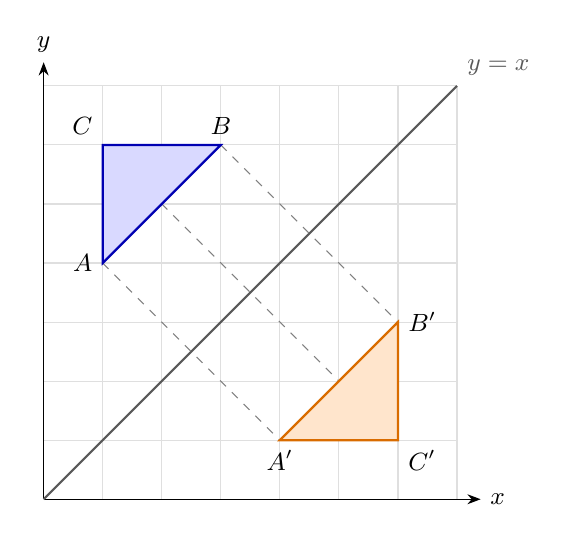
\begin{tikzpicture}[>={Stealth}, scale=0.75, every node/.style={font=\small}]
  % (x, y) maps to (y, x)
  \draw[gray!25] (0,0) grid (7,7);
  \draw[->] (0,0) -- (7.4,0) node[right] {$x$};
  \draw[->] (0,0) -- (0,7.4) node[above] {$y$};
  \draw[thick, gray!70!black] (0,0) -- (7,7) node[above right] {$y = x$};
  \draw[dashed, gray] (1,4) -- (4,1) (3,6) -- (6,3) (1,6) -- (6,1);
  \draw[thick, fill=blue!15, draw=blue!70!black] (1,4) node[left] {$A$} -- (3,6) node[above] {$B$} -- (1,6) node[above left] {$C$} -- cycle;
  \draw[thick, fill=orange!20, draw=orange!85!black] (4,1) node[below] {$A'$} -- (6,3) node[right] {$B'$} -- (6,1) node[below right] {$C'$} -- cycle;
\end{tikzpicture}
